\documentclass{beamer}
\usepackage{config}

%Information to be included in the title page:
\title[Présentation de la formation]{Présentation de la formation sur les Systèmes de Gestion de Versions}
\author{Florian Legendre}
\institute{Université de Poitiers}
\date{Année 2020 - 2021}
\logo{
\includegraphics[scale=0.1]{UP.png}}


%%% ============================================================= %%%
%%% ====================== Début des diapos ===================== %%%
%%% ============================================================= %%%

\begin{document}

\frame{\titlepage}

\begin{frame}
\frametitle{Table of Contents}
\tableofcontents[hideallsubsections]
\end{frame}


%% --------------------- %%
%%        SECTION        %%
%% --------------------- %%
\section{Qui suis-je?}

\begin{frame}
\frametitle{Qui suis-je?}
\begin{figure}[!htb]
        \begin{minipage}{0.65\textwidth}
            \begin{flushleft}
                Bonjour! Merci de l'intérêt que vous portez à cette formation et merci d'avoir répondu à l'enquête de besoins. Je m'appelle Florian Legendre et je suis étudiant en dernière année de licence informatique à l'Université de Poitiers.\\
                \medskip
                
                J'effectue actuellement un stage au laboratoire PPrime sous la responsabilité de M. Domalain et c'est dans le cadre de ce stage que je vous propose cette formation aux outils de gestion des versions.
            \end{flushleft}
        \end{minipage}
        \hfill
        \begin{minipage}{0.33\textwidth}
            \begin{flushright}
                
\includegraphics[scale=0.05]{images/me.jpg}
            \end{flushright}
        \end{minipage}
    \end{figure}
\end{frame}

\section{Pourquoi suivre cette formation?}
\begin{frame}
\frametitle{Pourquoi suivre cette formation?}
Vous avez certainement déjà géré des versions de documents à la main: une thèse, du code, un rapport, un document de recherche... \\
\medskip

Pour gérer ces versions vous avez probablement un document principal sur lequel vous écrivez et un dossier dans lequel vous stockez des versions de ce document (Exemple: doc\_V2.docx).\\
\medskip

Pour revenir à une version antérieur vous procédez ainsi:
\begin{center}
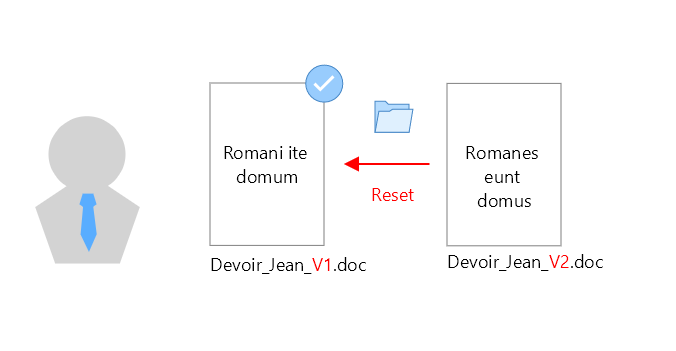
\includegraphics[scale=0.28]{images/pourquoi/firstScenario_diapo4.png}
\end{center}
\end{frame}

\begin{frame}
\frametitle{Pourquoi suivre cette formation?}
Cette méthode a ses avantages mais présente un certain nombre d'inconvénients, surtout quand vous travaillez à plusieurs sur de mêmes documents:\\
\medskip

\begin{tabular}{ | m{6em} | m{18em} | }
    \hline
    
    \textbf{Avantages} & \textbf{Inconvénients}\\
        
    \hline
    \begin{itemize}
    \item[+] Simple
    \end{itemize}
    & 
    \begin{itemize}
    \item[-] Pas toujours évident de savoir quelle version a apporté quel changement
    \item[-] Prend beaucoup de place!
    \item[-] Devient vite illisible si vous voulez faire des "versions alternatives"
    \item[-] Impossible quand on travaille à plusieurs de savoir qui a fait quoi et si on édite une partie d'un coéquipier
    \item[-] Prend du temps!
    \end{itemize}\\
    \hline
\end{tabular}


\end{frame}


\section{Qu'allez-vous apprendre?}
\begin{frame}{Qu'allez-vous apprendre?}
L'outil que je souhaite vous faire découvrir est un outil très puissant qui vous permettra de résoudre tous ces problèmes sur n'importe quel type de document texte.\\
\medskip

Cet outil s'appelle Git et il vous permettra de:
\begin{enumerate}
    \item Sauvegarder des versions
    \item Garder/Consulter un historique des versions 
    \item Comparer des versions/Revenir en arrière
    \item Faire des branches alternatives de versions
    \item Partager des versions
    \item Identifier des conflits d'éditions lors de collaborations
    \item Savoir à tout moment et très exactement qui a fait quoi
\end{enumerate}
\end{frame}

\begin{frame}[fragile]{Qu'allez-vous apprendre?}
Un dernier avantage de Git est qu'il suffit de l'apprendre une fois et vous maîtriserez tous les autres logiciels de gestion de versions du marché!
\end{frame}


\section{Comment allez-vous l'apprendre?}
\begin{frame}
\frametitle{Comment allez-vous l'apprendre?}
Pour vous faire découvrir cet outil j'ai choisi une approche:\\
\medskip

\begin{enumerate}
    \item Visuelle => Je vous fournirai de nombreux schémas et illustrations qui permettront une acquisition rapide des notions
    \item Concrète => Les séances, d'une durée de 1h, alterneront entre courts moments de théories et moments de pratiques sur machine
    \item Centrée sur vos besoins => Très vite nous verrons comment intégrer ce que vous apprendrez sur vos projets en cours
\end{enumerate}
\end{frame}


\section{Voulez-vous quelques exemples?}
\begin{frame}[fragile]{Voulez-vous quelques exemples?}
Git est un logiciel utilisant des commandes dont voici un exemple:
\begin{mdframed}[style=Bash]
    \begin{lstlisting}[style=Bash, caption={Contenu du dossier .git/}]
crex@crex:~/projects/test$ git init
Initialized empty Git repository in /home/crex/projects/test/.git/
    \end{lstlisting}
\end{mdframed}
\end{frame}

\begin{frame}{Voulez-vous quelques exemples?}
Ces commandes s'utilisent en boucles de travail. Aussi elles sont rapides à acquérir. Voici un exemple de boucle de travail:
\begin{center}
    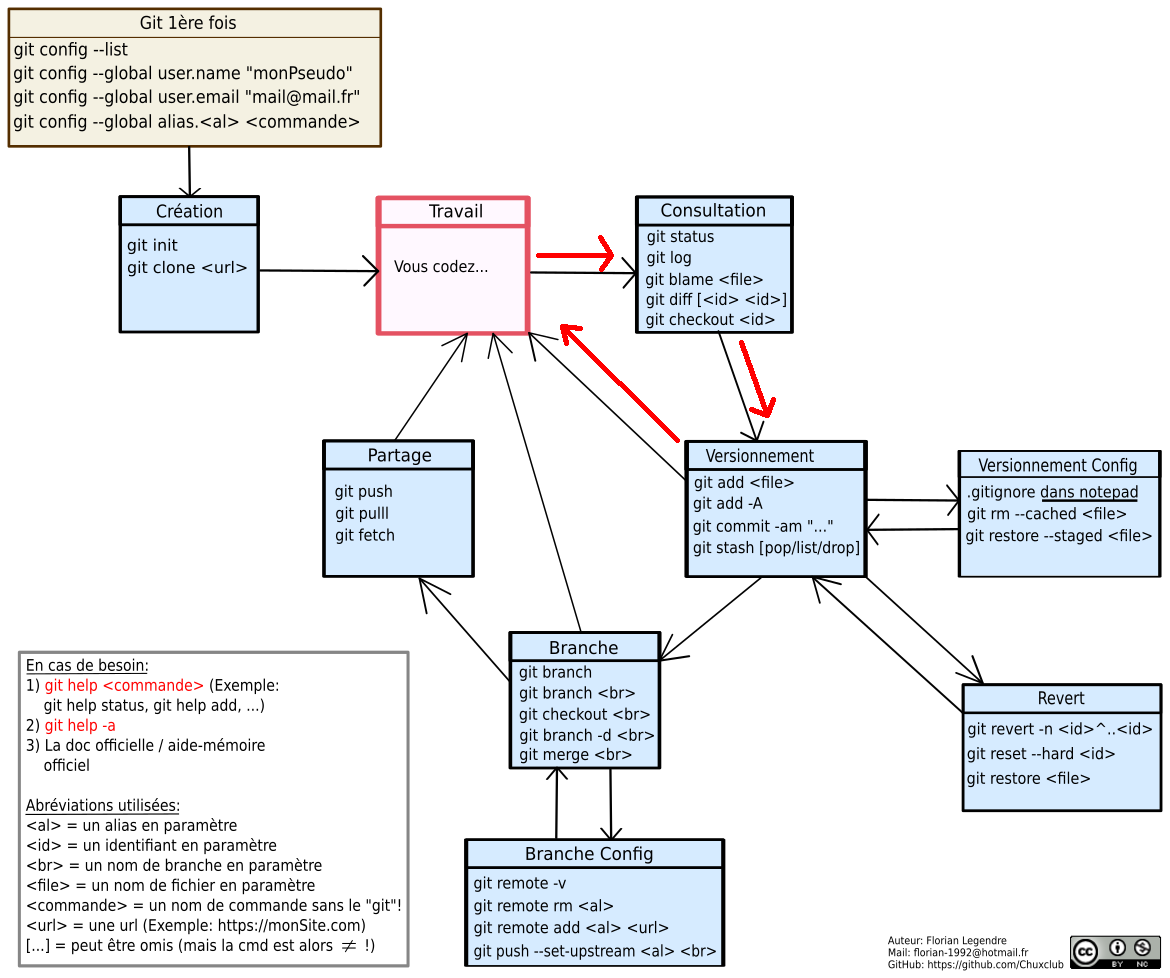
\includegraphics[scale=0.25]{images/comment/gitCommandFlow_localLoop.png}
\end{center}
\end{frame}

\begin{frame}[fragile]{Voulez-vous quelques exemples?}
Un exemple illustrant la détection automatique de conflits d'édition entre plusieurs collaborateurs:
\begin{mdframed}[style=Bash]
\begin{lstlisting}[style=Bash, caption={Exemple de détection automatique de conflit d'édition}]
<<<<<<< HEAD
VisuRepereMokka(markers.Potence,Rpotence_R0,c3d,'Rpotence_R0')
=======
VisuRepereMokla(markers.Potence,Rpotence_R0,c3d,'Rpotence_R0')
>>>>>>> travail_de_monOuma_collegue
\end{lstlisting}
\end{mdframed}
\end{frame}

\begin{frame}{Merci!}
    Merci d'avoir lu cette présentation, et j'espère vous dire à bientôt pour en découvrir davantage!
    \bigskip
   \begin{figure}[!htb] 
    \begin{minipage}{0.48\textwidth}
            \begin{center}
                
\includegraphics[scale=0.17]{images/git.png}
            \end{center}
        \end{minipage}
        \hfill
        \begin{minipage}{0.48\textwidth}
            \begin{center}
                
\includegraphics[scale=0.05]{images/github.png}
            \end{center}
        \end{minipage}
    \end{figure}
\end{frame}


\end{document}